%%%%%%%%%%%%%%%%%%%%%%%%%%%%%%%%%%%%%%%%%%%%%%%%%%%%%%%%%%%%%%%%%%%%%%%%%%%
\chapter{Introduction}
%%%%%%%%%%%%%%%%%%%%%%%%%%%%%%%%%%%%%%%%%%%%%%%%%%%%%%%%%%%%%%%%%%%%%%%%%%%

Pathfinding algorithms are methods of finding a path between two vertices in  
a graph. Most pathfinding problems are concerned with finding the shortest
path between two vertices, if there are more than one possible paths. There had 
been many pathfinding algorithms that had been developed throughout the years 
such as Minimum Spanning Tree (MST), Prim's Algorithm\cite{Prim1957}, and the A*
algorithm, which will be used in this paper.\cite{HartNilssonRaphael1968}

Functional programming is one of the major programming paradigms where computations 
are done by function composition. Along with this, purely-functional programming is 
a subparadigm of functional programming where there are no side-effects (e.g, variable mutability).
One of the major challenges of parallel programming is controlling the order of execution
to prevent \emph{race conditions}, which can often lead to bugs and are hard to maintain.
However, since purely-functional programming languages such as Haskell\cite{HaskellSite}
have no mutability and computations lead to the same result regardless of the order, they 
are a perfect candidate for writing parallel programs.\cite{Hammond2011} 
This research aims to find a parallel implementation of the existing A* pathfinding algorithm
using a purely-functional setting with attention to program performance in terms of time and space 
complexity. \cite{ZaghloulAlJami2017, WeinstockHolladay}
In turn, this helps in the advancement of different programming languages that feature 
functional programming and lambda expressions when it comes to purely-functional algorithms and data structures.

% Likewise, pure functions can be reasoned easier than functions with side-effects.
% Importing pure functions into other languages that can be used as proof assistants 
% such as Coq or Agda\cite{Breitner2018, SpectorZabusky2018, ElBakouny2017} is possible 
% and gives a better assurance of a bug-free parallel system.



% The Shortest Common Superstring (SCS) problem, known to be NP-Complete,
% seeks the shortest string that contains all strings from a given set.
% In this paper, we provide the summary of the problem and some of its characteristics.

% The SCS problem has been extensively studied for its
% applications in string compression and DNA sequence assembly \cite{Ma2009}.

% The superstring problem has applications to data storage,
%  specifically, data (string) compression \cite{Gallant1980}. 
% In many programming languages, a character string may be 
% represented by a pointer to that string. 
% The problem for the compiler is to arrange strings 
% so that they may be ``overlapped'' as much as possible.

% DNA sequence assembly is another  problem to which an SCS algorithm is known to apply.
% The $sequencing$ problem in molecular biology is to ``read'' a string of DNA,
% which can be viewed as a string over the alphabet \{A,C,G,T\}. Sequencing produces such a large number of fragments that
% almost all genome positions are covered by many fragments. This short fragments
% thus have large overlaps between other pieces. Hence, they can be given as an input to SCS algorithm.
% Figure \ref{fig:dna-overlap} shows an overlap graph consisting DNA reads (or fragments) as nodes. 



% \begin{figure*}
% \centering
% \fbox{
% \scalebox{0.65}{
% 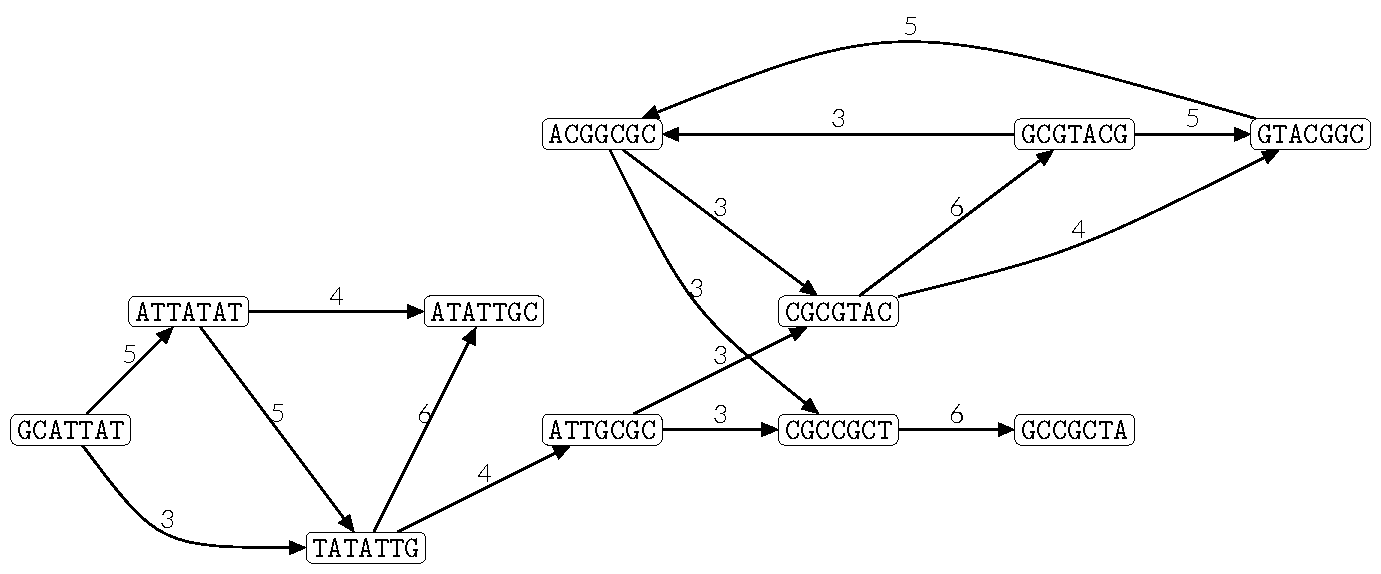
\includegraphics{fig-overlaps-dns-example}
% }}
% \caption{Sample overlap graph with each adjacent nodes 
% having at least $k = 3$ overlaps. The original string is \texttt{GCATTATATATTGCGCGTACGGCGCCGCTACA}.}
% \label{fig:dna-overlap}
% \end{figure*}	

% In \cite{Ma2009}'s paper, SCS was used to analyze DNA sequence assembly using
% a greedy algorithm. 

\section{Project Context}
The A* pathfinding algorithm is now mostly used as a pathfinding algorithm
for video games. While most video games are written in an imperative and 
object-oriented programming languages such as C\#, C++, and JavaScript, it is 
entirely possible to write video games in functional programming languages 
using a reactive functional programming paradigm. \cite{Cheong2006}

Functional programming had been getting more popular recently 
with more people using ReactJS, TypeScript, PureScript, and Scala.
However, imperative programming still dominates the industry, thus more algorithms 
are written for imperative programs. It can be observed that most algorithm books 
are written with imperative programming in mind such as \emph{Introduction to Algorithms}\cite{CLRS}, 
\emph{The Algorithm Design Manual}\cite{Skiena}, and \emph{The Art of Computer Programming}\cite{Knuth1997}.
Thus, the need for familiarity for functional approaches for some of the most popular 
algorithms should be discovered, since people are more familiar with imperative approaches 
and as such, it is moreoften used in developing video games than functional programming.

One reason for writing programs in a functional language is that 
pure functions are easy to reason about and can especially be aided with 
using a dependently-typed proof assistant such as Coq
or Agda.\cite{Breitner2018,SpectorZabusky2018,ElBakouny2017}.
Programs written in functional programming can be easily proven out 
by reasoning about the smaller components and composing two or more proven 
functions into a single function and it should also give the correct result with respect to the input,
provided that the algorithm is correct. \cite{AbelBenkeBove2005}

\section{Purpose and Description}

This research aims to utilize the existing A* pathfinding algorithm
\cite{ZaghloulAlJami2017,WeinstockHolladay}
and find a way to develop a reasonably-efficient purely-functional 
implementation of the algorithm using parallel data structures such 
as STMs or MVars\cite{Marlow2013}.  

The A* Pathfinding algorithm is used heavily in video games, telephone traffic, 
and other graph traversal problems\cite{HartNilssonRaphael1968}. This research 
aims to aid in the development of video games using the functional 
programming paradigm in the future as video game development is dominated 
by imperative languages.

\section{Objectives}
The research aims to find an efficient parallel implementation of the A* pathfinding 
algorithm using a purely-functional programming language such as Haskell. Likewise, 
concrete comparisons between the number of cores and logical threads will be used to measure 
the most efficient performance runtime of the algorithm.

The researchers aim to create two programs that will be used in the research. A generator program
that will generate an arbitrary-sized maze that will be relatively hard to solve without the aid 
of computers in a short amount of time.\cite{Buck2015} And a solver program will be written for translating the output 
of the maze generator to an algebraic graph that the A* algorithm can understand. The solver
program will be a browser-based application that will show the maze graphically and the generated 
path when the algorithm terminates. This pathfinding program must have an efficient performance while solving the maze. 
To measure the performance of the program, the application ThreadScope will be used to monitor the thread and
core activities while the program is being run. \cite{ThreadScope}
% \vfill\eject
\section{Scope and Limitations}

The research will only cover solvable-mazes as the A* algorithm does not halt when there is no reachable end goal (e.g,
the start vertex and end vertex lie on different components of the graph).\cite{HartNilssonRaphael1968} Likewise, there will be no generality
and all programs will be written in Haskell. Translation to other functional programming languages is not a priority and, thus,
lambda notation will not be used. Other concurrent data structures besides MVar and Software Trasnactional Memory will not be utilized. The 
implementation of the graph that the research will use will be Algebraic Graphs.\cite{Mokhov2017}

The concrete implementation and analysis is planned to be tested only on four CPUs such as Intel Core i7-9750H and AMD Ryzen 5 3500x.
Other CPU architectures are not planned to be tested on.